\chapter{Implementación digital} \chapterlabel{Informe/7-ImplementacionDigital} \label{cap:Implementacion digital}

En este capítulo se realiza el diseño de un compensador y estimador en el dominio digital para ser implementados en un microcontrolador que se conecta de manera externa a la placa de control. Para el primero se sigue la misma estrategia que se utiliza en la etapa de compensación analógica, descripta en el capítulo \ref{cap:Compensador Analogico}, pero con las consideraciones necesarias para trabajar con sistemas discretos. Para el segundo, se diseña un algoritmo encargado de obtener el valor de la distancia de separación $Y_g$ a partir de los valores obtenidos al muestrear la tensión entregada por el sensor de efecto Hall.

Por otra parte, se diseñan los circuitos de interfaz encargados de muestrear, reconstruir y adaptar los niveles de tensión de las señales que interactúan entre la placa de control y el microcontrolador.


\section{Descripción general}

\noindent La implementación digital consiste en realizar la estimación de posición y el control de la planta por medio de un microcontrolador. Se utiliza un kit de desarrollo basado en el microcontrolador STM32F072, que contiene un DAC y un ADC, ambos de 12 bits y $3.3\:V$ de referencia. 

\noindent En la figura \ref{fig:diag-en-bloques-digital} se muestra un diagrama en bloques general de la implementación digital del sistema. Es posible observar que se ingresa al microcontrolador a través de un ADC, con una tensión de referencia ($V_{ref}$) proporcional a la distancia de separación deseada. Esa posición de referencia es comparada con la posición estimada $Y(z)$ y el resultado $e(z)$ es afectado por el compensador digital $C(z)$. Por medio de un DAC, la salida del compensador ingresa al controlador de corriente $G_{iL}(s)$, el cual actúa sobre la planta $G_P(s)$, y modifica la distancia de separación.

\noindent Por medio de un ADC y el sensor de efecto Hall, se muestrea una tensión proporcional a la corriente que circula por el electroimán. De esta forma, es posible obtener una posición estimada $Y(z)$ al multiplicar esta tensión por la transferencia $H(Z)$.


\begin{figure}[H]
	\centering
	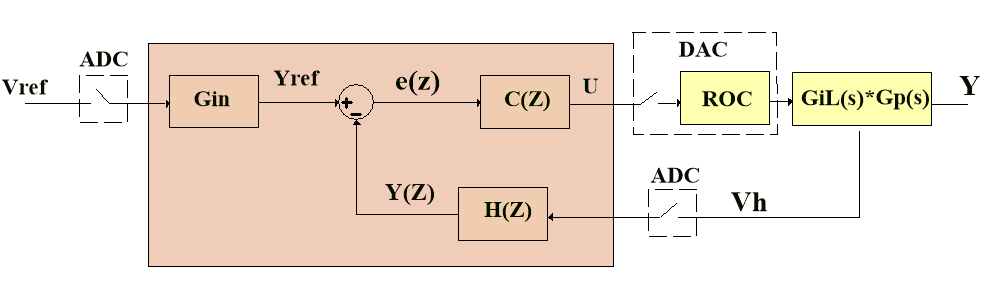
\includegraphics[scale=0.5]{Diagrama-en-bloques-digital.png}
	\caption{Diagrama en bloques de la implementación digital.}
	\label{fig:diag-en-bloques-digital}
\end{figure}
\colorbox{red}{dejar un solo diagrama y cambiar lo de abajo}
\noindent Abstrayéndose de la matemática que se realiza dentro del microcontrolador para la estimación de posición, se puede simplificar el diagrama al que se muestra en la figura \ref{fig:diag-en-bloques-digital-simplif}, en la que:

\begin{equation} 
	G_T(s) = G_P(s) * G_{iL}(s).
\end{equation}

\begin{figure}[H]
	\centering
	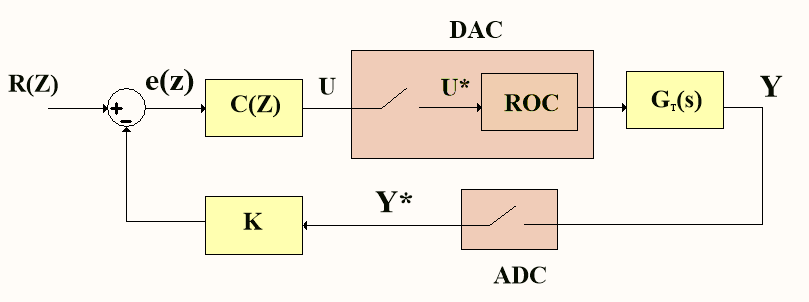
\includegraphics[scale=0.5]{Diagrama-en-bloques-digital-simplificado.png}
	\caption{Diagrama en bloques de la etapa digital simplificado.}
	\label{fig:diag-en-bloques-digital-simplif}
\end{figure}


\section{Determinación de la frecuencia de muestreo}

\noindent Se desea realizar una estimación de la posición del electroimán $Y(z)$  a partir de las muestras tomadas por el ADC de la tensión de salida del sensor de efecto Hall.

\noindent La forma de onda de la salida del sensor es triangular y presenta una frecuencia variable en función de la distancia de separación. Se puede calcular como:

\begin{equation} \label{eq_frecuencia-de-muestreo}
	F_{planta}(Y_g)=\frac{V_{BUS}}{2 * L(Y_g) * \Delta I_H}
\end{equation}


 Al aplicar en la ecuación \ref{eq_frecuencia-de-muestreo} los valores de inductancia ($L\:[mHy]$) obtenidos en las mediciones realizadas sobre el electroimán (ver tabla \ref{tab_mediciones_inductancia}), se calcula la frecuencia de conmutación  $(F_{planta}\:[Hz])$. Los resultados se muestran en la tabla \ref{frecuencias-calculadas}.



\begin{table}[H]
	\begin{center}
		\begin{tabular}{| c | c | c |}
			\hline
			$Y_g\:[mm]$ & $L\:[mHy]$ & $F_{planta}\:[Hz]$\\ \hline
			2 & 22.64 & 1060\\ \hline
			3 & 18.8 & 1276\\ \hline
			4 & 16.44 & 1459\\ \hline
			5 & 14.9 & 1632\\ \hline
		\end{tabular}
		\caption{Valores de frecuencia calculados a partir de las mediciones de inductancia realizadas.}
		\label{frecuencias-calculadas}
	\end{center}
\end{table}


\noindent Para la estimación de la posición es necesario medir la pendiente de la onda triangular. Por lo tanto, para reconstruir su forma de onda es necesario que la frecuencia de muestreo del ADC sea al menos el doble de la frecuencia de la 5° armónica para el caso de la mayor frecuencia. Por lo tanto, se adopta 2.5 veces. Es decir:

\begin{equation} 
	F_S \geq 2.5 * 5 * f_{max} \Rightarrow  F_S \geq 2.5 * 5 * 1666 Hz \Rightarrow F_S \geq 20825 Hz
\end{equation}

\noindent De esta forma, se adopta una frecuencia de muestreo para el ADC de  $25 \:kHz$. Por lo tanto, es posible obtener 15 muestras en un período de la triangular para el caso de la frecuencia máxima. Como la señal crece o decrece durante medio ciclo, se pueden tomar 7 muestras para identificar la pendiente. En el caso de que la señal presente la frecuencia mínima, se pueden tomar 23 muestras en un ciclo, que se traduce en 11 muestras para la pendiente de subida o bajada. 


\section{Adquisición y procesamiento de las muestras}

\noindent Al considerar el caso de máxima frecuencia, en el que solo se pueden tomar 7 muestras durante el tiempo de crecimiento o decrecimiento, se describe el procedimiento para determinar la posición estimada.


\begin{figure}[H]
	\centering
	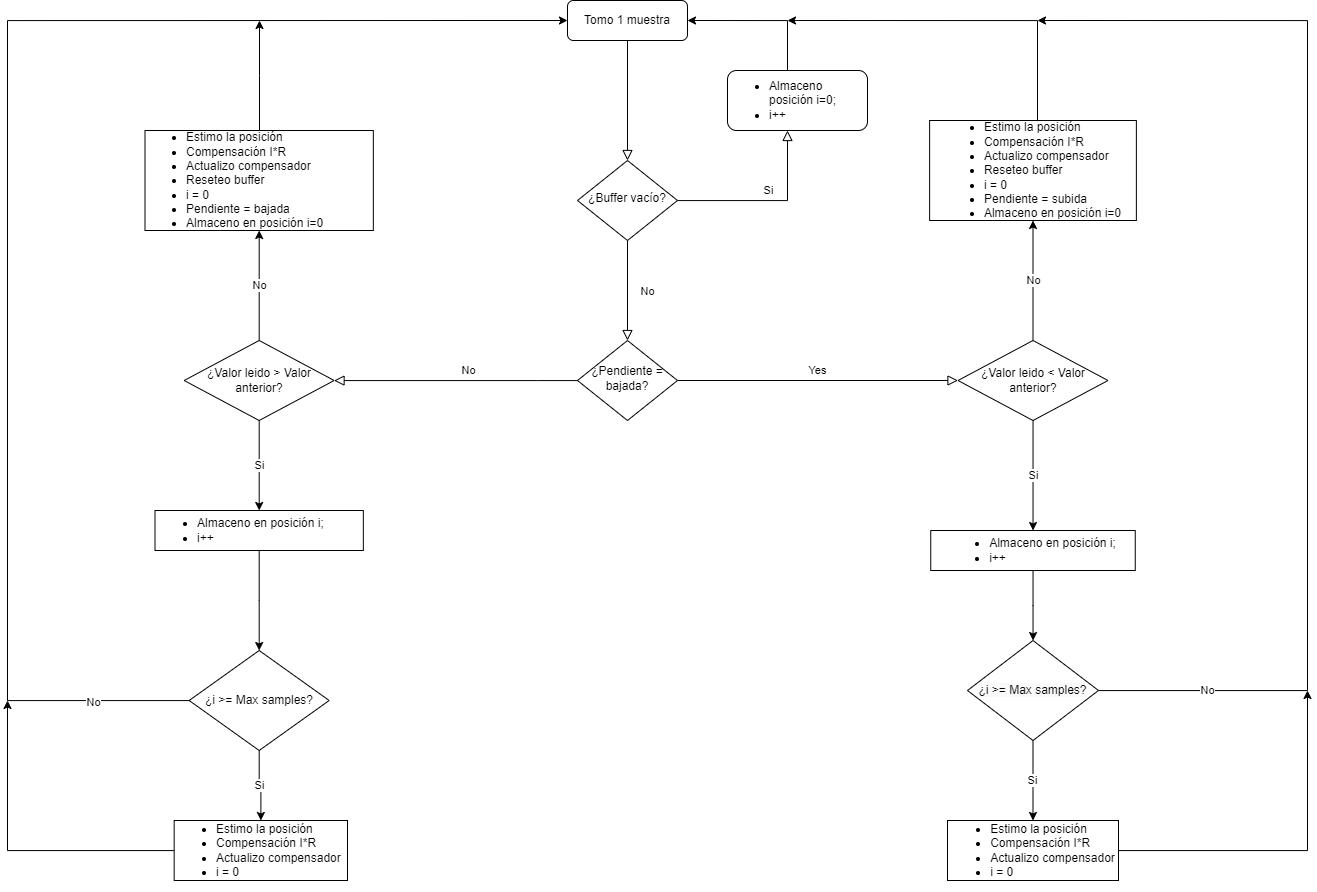
\includegraphics[scale=0.55]{Procesamiento-muestras-adquiridas.png}
	\caption{ Diagrama de flujo del procesamiento de las muestras adquiridas.}
	\label{fig:procesamiento-muestras-adquiridas}
\end{figure}


\noindent Como se observa en el diagrama de flujo de la figura \ref{fig:procesamiento-muestras-adquiridas}, cada muestra de tensión tomada del sensor de efecto Hall, se almacena en un buffer de 7 posiciones. Para poder discernir entre pendientes de bajada y de subida, se verifica en cada muestra si el valor leído es mayor o menor al almacenado en la posición anterior. En caso de que sea mayor al anterior, significa que se está muestreando la pendiente positiva de la onda triangular. La distinción entre pendientes positivas y negativas es importante puesto que permite aplicar la compensación de la resistencia interna al igual que se realiza en el estimador analógico. 

\noindent Cada vez que el buffer se completa, se realiza el cálculo de la derivada con el valor máximo y mínimo almacenado. Con este resultado, se hace la estimación de la posición y se actualiza la entrada al compensador digital.

\noindent En caso de haber completado las 7 posiciones del buffer y la pendiente persiste con el mismo signo, el buffer comienza a llenarse nuevamente desde la posición inicial, sobrescribiendo los valores de mayor vejez. Por lo tanto, pueden ocurrir dos situaciones. La primera es que se detecte un cambio de pendiente antes de completar nuevamente el buffer, con lo cual se calcula la derivada con los valores extremos almacenados teniendo en cuenta el tiempo transcurrido ($K$ períodos de muestreo), y se actualiza la entrada al compensador. La segunda, es que se vuelva a completar el buffer, en cuyo caso también se hace la actualización. La diferencia entre estas dos situaciones es el tiempo transcurrido hasta que se obtiene nueva estimación. En este último, se hace cada 7 períodos de muestreo mientras que en el primero se realiza en “N” períodos luego de la última actualización, siendo “N” la cantidad de muestras que se almacenaron en el buffer incompleto.

\noindent Luego de detectar un cambio de pendiente, el
proceso vuelve a iniciar con el buffer vacío.

\noindent Al utilizar este método de estimación, puede ocurrir que se obtenga una nueva estimación en 7 periodos de muestreo del ADC, o incluso en menos. Por lo tanto se tiene un estimador de posición con frecuencia de actualización variable. Esto es importante al momento de diseñar un compensador digital para el sistema. Para hacerlo, se debe considerar el caso en que la frecuencia de actualización es la menor, por lo tanto el compensador digital se debe diseñar con una frecuencia de muestreo de $25/7 \:kHz = 3.5\:kHz$.

\section{Estimación digital de la posición}

A partir de la expresión \ref{eq_di-dt_lineal}, que relaciona la distancia de separación con la pendiente de la corriente en el electroimán, se despeja la posición ($Y_g$) y se obtiene:

\begin{equation} \label{eq_yg_vs_derivada}
	Y_g = 5.136*10^{-6}*|\frac{di_L}{dt}|- 3.472*10^{-3} [m]
\end{equation}

\noindent Es importante notar que la resistencia interna del electroimán ($R_L$) genera una caída de tensión cuando circula corriente. Esta caída provoca que la tensión efectiva aplicada sobre la inductancia sea distinta para el semiciclo de subida que para el de bajada. De esta forma, la onda triangular presenta diferentes pendientes (en valor absoluto) para cada caso. Esta se representa como $(\frac{di_L}{dt})_{Real}$ y es la que se mide al utilizar el ADC. Es decir:


\begin{equation} \label{eq_derivada_real}
	(\frac{di_L}{dt})_{Real}=(\frac{di_L}{dt})_{Teorica}-\frac{R_L*I_L}{L(Y_g)}
\end{equation}

Por lo tanto al despejar la derivada teórica de la expresión \ref{eq_derivada_real} se obtiene:

\begin{equation} \label{eq_derivada_teorica}
	(\frac{di_L}{dt})_{Teorica}=(\frac{di_L}{dt})_{Real}+\frac{R_L*I_L}{L(Y_g)}
\end{equation}


\noindent Al aproximar la derivada real como la resta entre la muestra de corriente en un instante menos el anterior sobre el período de muestreo y al utilizar \ref{eq_derivada_teorica} en \ref{eq_yg_vs_derivada}, se obtiene:

\begin{equation} 
	Y_g[n] = 5.136*10^{-6}* |\frac{I_L[n]-I_L[n-K]}{K*T_S}+\frac{R_LDD*I_L[n]}{L(Y_g)[n-1]}| - 3.472*10^{-3} [m]
\end{equation}

\noindent Al considerar a $V_h$ como la tensión entregada por el sensor de efecto Hall, proporcional a la corriente que circula por el electroimán multiplicada por una ganancia $K_h$ de $53.3\:mV/A$, con  ($\hat{V_h}$)  correspondiente a la componente alterna de tensión y ($\bar{V_h}$) a la continua, resulta:


\begin{equation} 
	V_h[n] = \bar{V_h}[n] + \hat{V_h}[n] = K_h * (\bar{I_L}[n] + \hat{I_L}[n])
\end{equation}

\noindent Para la estimación de la posición se utiliza el término de alterna mientras que para compensar el error introducido por la resistencia interna del electroimán se utiliza el de continua. Por lo tanto, se obtiene:

\begin{equation}
	\resizebox{.8\hsize}{!}
	{
	$Y_g[n] = 5.136*10^{-6}*|\frac{\hat{V_h}[n]-\hat{V_h}[n-K]}{K*K_h*T_S} + \frac{R_L*\bar{V_h}[n]}{K_h*L(Y_g)[n-1]}|-3.472*10^{-3}[m]$
	}
\end{equation}

\noindent El término $\bar{V_h}[n]$ se obtiene de sensar el valor medio de tensión entregado por el sensor de efecto Hall mediante un canal del ADC.

\noindent Por otro lado, el valor de $L(Y_g)[n-1]$ se obtiene al aplicar el valor estimado de posición anterior en la ecuación \ref{eq_inductancia}. El cálculo de esta expresión se obtiene a partir de la linealización de la inductancia en función de las mediciones realizadas sobre el electroimán.


\begin{equation} \label{eq_inductancia}
	L(Y_g)[n] = -2.56*Y_g[n]+0.0271\:Hy
\end{equation}

\noindent Por lo tanto, la ecuación correspondiente en el tiempo discreto resulta:

\begin{equation}
	\resizebox{.8\hsize}{!}
	{
	$Y_g[n] = 5.136*10^{-6}*|\frac{\hat{V_h}[n]-\hat{V_h}[n-K]}{K*K_h*T_S} + \frac{R_L*\bar{V_h}[n]}{K_h*(2.56*Y_g[n-1]+0.0271)}|-3.472*10^{-3}\:[m]$
	}
\end{equation}

\begin{equation}
	\resizebox{.8\hsize}{!}
	{
	$
	Y_g[n] = 96.3*10^{-6}*|\frac{\hat{V_h}[n]-\hat{V_h}[n-K]}{K*T_S} + \frac{R_L*\bar{V_h}[n]}{(2.56*Y_g[n-1]+0.0271)}|-3.472*10^{-3}\:[m]
	$
	}
\end{equation}


\noindent El número de muestras está representado por ``n''. Es decir, $V_h[n]$ se refiere a la muestra más reciente en el buffer y $V_h[n-K]$ a la más vieja.

Es importante notar que los coeficientes del estimador deben calcularse justo antes de realizar una nueva estimación,  en función de la cantidad de muestras que se utilizan para el cálculo de la pendiente. Si bien el estimador presenta una frecuencia de actualización variable, los coeficientes del compensador digital no se ven modificados ya que se calculan teniendo en cuenta la frecuencia de actualización más lenta.

\noindent Por otro lado, el bloque $H_D$ mostrado en la figura \ref{fig:diag-en-bloques-digital-simplif} resulta en una transferencia unitaria.

\section{Resolución en posición}

\noindent Una variación de posición ($\Delta Y_g$) produce un cambio de inductancia ($\Delta L[Y_g]$) que se traduce en un cambio de frecuencia ($\Delta F_{planta}$). Para poder detectar el mínimo cambio de posición en un período de muestreo se debe tener una resolución tal que permita discernir ese cambio de frecuencia.


\noindent A partir de la expresión linealizada de la inductancia \ref{eq_induct_practica} y la ecuación \ref{eq_frecuencia-de-muestreo} es posible obtener el valor de frecuencia para una separación de $Y_g=2.1\:mm$. Esta resulta en $F_{planta}[2.1\:mm] = 1104.8\:Hz$. De esta forma, al conocer el valor de frecuencia para $2\:mm$, el cual es de $F_{planta}[2\:mm] = 1060\:Hz$, es posible obtener la variación de frecuencia para un ($\Delta Y_g$) mínimo de  $0.1\:mm$. Este valor puede obtenerse como:

\begin{equation} 
	\Delta F_{planta} = F_{planta}[2.1\:mm] - F_{planta}[2\:mm] = 44.8\:Hz
\end{equation}

\noindent Las pendientes para el peor caso se da con la menor variación de tensión entre muestras. Es decir, para el caso de frecuencia mínima. En la ecuación \ref{eq_pendiente} se muestra el cálculo de la pendiente de la onda triangular en función de la frecuencia de conmutación.

\begin{equation} \label{eq_pendiente}
	P(F_{planta}) = \frac{\Delta V}{T_{SW}/2} = 2*K_h*\Delta i_L*F_{planta} = 2 * 0.0533 * 0.5 * F_{planta}
\end{equation}

\noindent A partir de la ecuación \ref{eq_pendiente} es posible obtener el valor de la pendiente para la mínima frecuencia de conmutación y la de su incremento correspondiente a una variación en la posición de $0.1\:mm$. Esta situación se representa en la figura \ref{fig:variacion-de-pendiente}.

\begin{equation} 
	\begin{aligned}
		&P(f_{SW_{min}}) = 56.49\:[V/s] \\
		&P(f_{SW_{min}} + \Delta F_{planta}) = 58.89\:[V/s] \\
	\end{aligned}
\end{equation}

\begin{figure}[H]
	\centering
	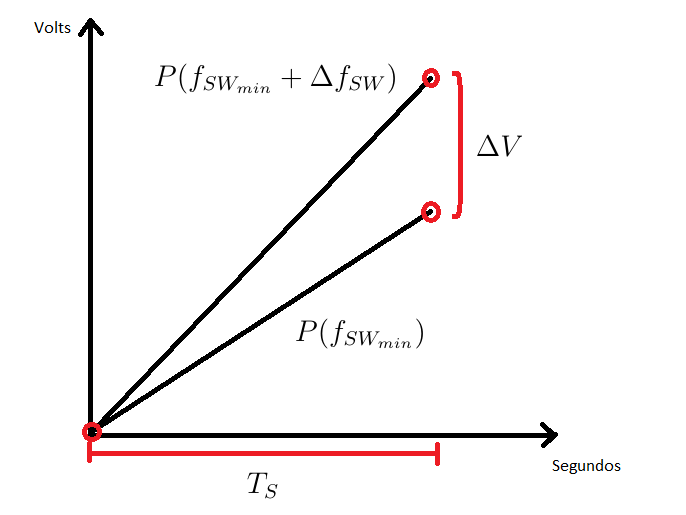
\includegraphics[scale=0.5]{Variacion-de-pendientes.png}
	\caption{Variación de pendiente ante mínimo cambio de posición.}
	\label{fig:variacion-de-pendiente}
\end{figure}

\noindent Por lo tanto, para poder diferenciar las pendientes, la resolución del ADC debe ser menor o igual a $\Delta V$.

\begin{equation} 
	\begin{aligned}
		V1 &= P(f_{SW_{min}} + \Delta F_{planta})* T_S \\
		V2 &= P(f_{SW_{min}})* T_S \\		 
	\end{aligned}
\end{equation}

\noindent Al considerar $F_s = 25\:kHz$:

\begin{equation} 
	\Delta V_{ADC} = T_S * [P(f_{SW_{min}} + \Delta F_{planta}) - P(f_{SW_{min}})] = 96\:\mu V
\end{equation}



\noindent Este resultado indica que, al usar un ADC de 12 bits, se necesitaría una tensión de referencia $V_{ref} = 0.39\:V$. Sin embargo, este valor resulta demasiado bajo y no sirve si se quiere medir la tensión de salida del sensor de efecto Hall de manera directa. Por lo tanto, se decide diseñar un circuito que permita realizar la estimación manteniendo la tensión de referencia en $3.3\:V$

\noindent La corriente que circula por el electroimán presenta una componente de continua y otra de alterna. La primera excursiona entre $0\:A$ y $30\:A$ mientras que la segunda varía entre $\pm 250\:mA$ en torno al valor medio, con forma de onda triangular. Por lo tanto, se realiza una adquisición separada de ambas componentes de la tensión de salida del sensor de efecto Hall con el ADC, sin el \textsl{set-point} de $2.5\:V$.

\noindent A la  salida del sensor de efecto Hall se obtiene una señal cuyo valor medio varía entre $0\:V$ y $1.6\:V$, y un valor de alterna de $26.7\:mV_{pp}$.

\noindent Debido a que el ADC permite una excursión entre $0\:V$ y $3.3\:V$, la máxima ganancia posible es de 60 veces para la componente de alterna. Por otro lado, para medir con la resolución en posición deseada de $0.1\:mm$ se debe amplificar la señal triangular 9 veces como mínimo.

\noindent Por lo tanto, se adopta una ganancia de 50, y se obtiene una excursión máxima de $3.17\:V$ (es decir, $0.67\:V$ sobre el \textsl{set-point}).


\noindent Las características del circuito son:

\begin{itemize}
	\item Ganancia: 50
	\item \textsl{set-point} de $2.5\:V$
	\item Frecuencia de corte inferior: $100\:Hz$
	\item Frecuencia de corte superior: $12,5\:kHz$
\end{itemize}

\noindent Al considerar la ganancia elegida,  la pendiente de la onda triangular resulta:

\begin{equation} 
	P(F_{planta}) = 50 * [0.0533 * 0.5 * (F_{planta}*2)]\:[\frac{V}{s}]
\end{equation}

\noindent Al reemplazar para el incremento de frecuencia se obtiene: 

\begin{equation} 
	\begin{aligned}
		&P(f_{SW_{min}}) = 2824.9 \: [\frac{V}{s}]\\
		&P(f_{SW_{min}} + \Delta F_{planta}) = 2944.29 \: [\frac{V}{s}]\\		 
	\end{aligned}
\end{equation}

\noindent Por lo tanto, resulta:


\begin{equation} 
	\resizebox{.8\hsize}{!}
	{
	$\Delta V_{ADC} = T_S * [P(f_{SW_{min}} + \Delta F_{planta}) - P(f_{SW_{min}})] = 0.1177\:V - 0.1129\:V = 4.7\:mV$
	}
\end{equation}


\noindent De esta manera, como la resolución del ADC es de $0.8\:mV$, resulta suficiente para identificar el mínimo cambio de pendiente.


\section{Acondicionamiento de señales para el ADC}

\subsection{Referencia de posición}

\noindent Para indicar al microcontrolador la distancia de separación deseada se utiliza una señal continua como referencia que se ajusta desde un potenciómetro ubicado en la placa de control  e ingresa al circuito mostrado en la figura \ref{fig:circuito-ref-posicion}. Esta señal de referencia es también utilizada por el compensador analógico. Debido a que entrega una tensión entre $3.96\:V$ y $4.69\:V$, se implementa un circuito de acondicionamiento.

\noindent A la señal de entrada se le resta el \textsl{set-point} de $2.5\:V$, para lograr señales que van desde $1.42\:V$ a $2.2\:V$. Luego, dentro del microcontrolador, se debe mapear el valor leído por el ADC con la posición deseada utilizando la ganancia del estimador analógico según la expresión \ref{eq_y-ref-dig}. Además se implementa un filtro \textsl{anti-aliasing} con frecuencia de corte en $9.9\:kHz$.

\begin{equation} \label{eq_y-ref-dig}
	Y_{ref}\ =\frac{Vpo{s_{ref}}_{ADC}\ +\ 2.5\:V}{259.6}\:[m]
\end{equation}

\begin{figure}[H]
	\centering
	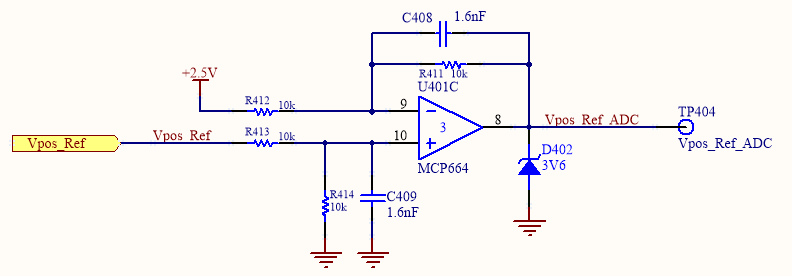
\includegraphics[scale=0.5]{Circuito-ref-posicion.png}
	\caption{Circuito acondicionador para referencia de posición.}
	\label{fig:circuito-ref-posicion}
\end{figure}

\subsection{Componente  alterna de corriente del electroimán}

\noindent Para obtener solamente la componente alterna de la corriente, se implementa un circuito con característica pasa-banda que se muestra en la figura \ref{fig:componente-corriente-alterna}. La frecuencia de corte inferior  es de $100\:Hz$, con el objetivo de eliminar el valor medio de señal. Por otro lado, la superior es de $12\:kHz$, que actúa como filtro \textsl{anti-aliasing}. Luego, la salida es amplificada con una ganancia de 50 veces (para mejorar la medición de la pendiente por el ADC) y se agrega un \textsl{set-point} de $2.5\:V$.

\begin{figure}[H]
	\centering
	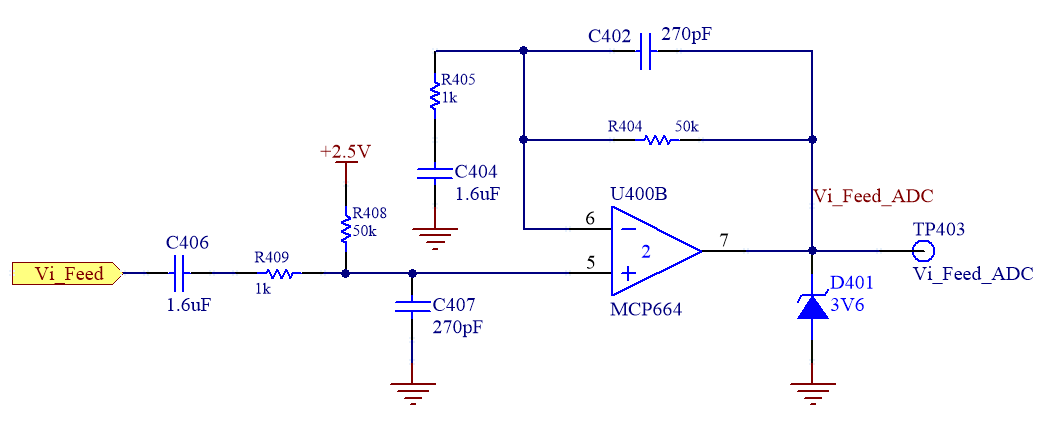
\includegraphics[scale=0.5]{Componente-corriente-alterna.png}
	\caption{ Circuito acondicionador para componente alterna de corriente del electroimán.
	}
	\label{fig:componente-corriente-alterna}
\end{figure}

\subsection{Componente  contínua de corriente del electroimán}

\noindent Para obtener la componente de contínua se utiliza un filtro pasa-bajos con frecuencia de corte en $106\:Hz$. Se eligió esta frecuencia para que se ubique por lo menos una década por debajo de la frecuencia fundamental de la onda triangular. La implementación circuital puede observarse en la figura \ref{fig:componente-corriente-continua}


\begin{figure}[H]
	\centering
	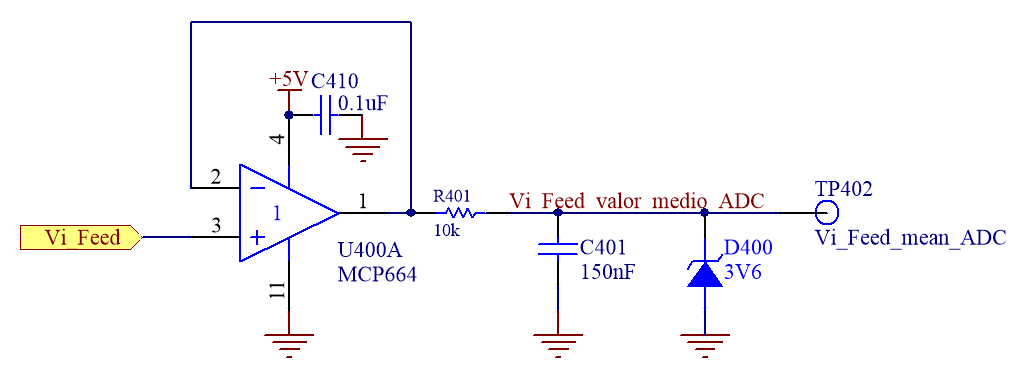
\includegraphics[scale=0.5]{Componente-corriente-continua.png}
	\caption{Circuito acondicionador para componente continua de corriente del electroimán.
	}
	\label{fig:componente-corriente-continua}
\end{figure}

\section{Acondicionamiento de señales para el DAC}

\noindent Para convertir los valores digitales de la estimación de posición y de la compensación al dominio analógico, se utiliza el DAC del microcontrolador. La tensión entregada es afectada por una circuitería de filtrado, ganancia y protección como se muestra en las figuras \ref{fig:DAC-compensador} y \ref{fig:DAC-estimador}. Debido a que el DAC se actualiza con una frecuencia mínima de $3.5\:kHz$, se utilizan filtros con frecuencia de corte en $1.75\:kHz$.

\noindent Por otro lado, como el controlador de corriente funciona con tensiones de hasta $5\:V$ en su entrada y el compensador fue diseñado teniendo en cuenta este nivel de tensión, se agrega una ganancia por firmware de $0.66$, mapeando así los $5\:V$ a $3.3\:V$, que es la máxima tensión entregada por el DAC. Luego, para compensar esta ganancia y no afectar a la transferencia de la planta, se la afecta por un factor de $\frac{5V}{3.3V}$ por medio del circuito de acondicionamiento.

\noindent De esta forma, se logra convertir correctamente la señal digital en analógica.


\begin{figure}[H]
	\centering
	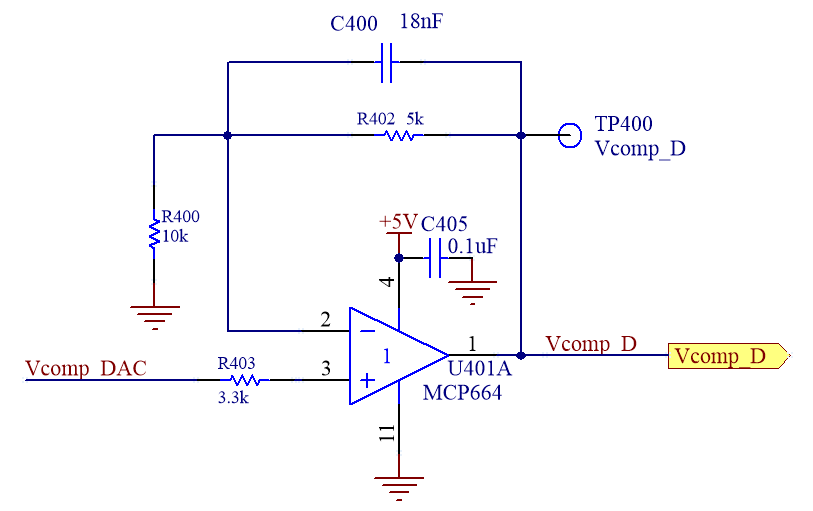
\includegraphics[scale=0.5]{DAC-compensador.png}
	\caption{Circuito acondicionador para la salida del DAC correspondiente al compensador.}
	\label{fig:DAC-compensador}
\end{figure}

\begin{figure}[H]
	\centering
	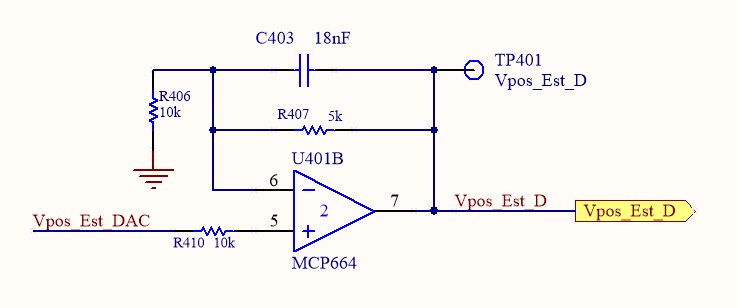
\includegraphics[scale=0.5]{DAC-estimador.png}
	\caption{Circuito acondicionador para la salida del DAC correspondiente al estimador digital.}
	\label{fig:DAC-estimador}
\end{figure}

\section{Diseño del controlador digital}

Para poder diseñar un compensador digital para un sistema continuo, se puede utilizar la transformada bilineal para poder aplicar técnicas de compensación´´on analógica en un sistema discreto.

 \colorbox{red}{Redactar bien esta parte}
Por medio de la transformada bilinal es posible diseñar un compensador en el dominio analógico y luego, con su transformada inversa, obtener el compensador en el dominio discreto. Por lo tanto se decide usar la misma estrategia utilizada en el compensador analógico, planteando dos lazos de realimentación: uno interno y otro externo. El primero con el objetivo de estabilizar la planta y el segundo para mejorar la respuesta temporal del sistema.  

\subsection{Transferencias de la planta y del controlador de corriente}

\noindent Para el an\'{a}lisis del compensador digital se parte de las transferencias de la planta $G_P(s)$ y del controlador de corriente $G_{iL}(s)\ $ en dominio anal\'{o}gico para una masa de $30 \:kg$.

\begin{equation} 
	\begin{aligned}
		G_T(s)[M=30kg]&=G_P(s)*G_{iL}(s)&=\frac{-87.7}{\ (s-70)\ (s+70)\ (s+12.17)}\\
	\end{aligned}
\end{equation}

\noindent Al aplicar la transformada z por invarianza al impulso, con una $f_s=3.5\:kHz$, se obtiene:

\colorbox{red}{Escribir la expresión de la transformada bilienal}

\begin{equation} 
	G_T(Z)[M=30\:kg] =\frac{-3.2057*10^{-10}(z+3.729)(z+0.2677)}{(z-0.9966)(z-0.9806) (z-1.02)}
\end{equation}

\noindent Luego, al usar la transformada bilineal para volver al dominio anal\'{o}gico:

\begin{equation}
	\resizebox{.8\hsize}{!}
	{
		$G_T(w)[M=30\:kg]\ \ =\frac{-8.0207*10^{-11}(w-1.238*10^4)(w-7143)(w+1.237*10^4)}{\ (w-70)\ (w+70)\ (w+12.17)}$
	}
\end{equation}


\noindent Con las expresiones en $[w]$ es posible diseñar un controlador en el dominio analógico y luego transformarlo al digital.

\subsection{Diseño del compensador}

Se decide usar la misma estrategia utilizada en el compensador analógico, planteando dos lazos de realimentación: uno interno y otro externo. El primero con el objetivo de estabilizar la planta y el segundo para mejorar la respuesta temporal del sistema.  

Por lo tanto, se plantea el diagrama en bloques de la figura \ref{fig:diag-en-bloques-comp_digital}


\begin{figure}[H]
	\centering
	\scalebox{0.8}{\tikzset{%
	buffer/.style={
		draw,
		shape border rotate=270,
		regular polygon,
		regular polygon sides=3,
		fill=blue!20,
		node distance=2cm,
		minimum height=4em
	}
}

\tikzstyle{block} = [draw, fill=blue!20, rectangle, 
minimum height=2.5em, minimum width=3em]

%Acá se define eñ diagrama en bloques completo
\begin{tikzpicture}[auto, node distance=1cm,>=latex']
	% We start by placing the blocks
	\node [input, name=input] {};
	\node [buffer, right=of input](F){F};
	\node [sum, right of=F, node distance=1.5cm] (suma_externa) {+};
	\node [block, right=of suma_externa] (externo) {$G_{ext}(w)$};
	\node [sum, right=of externo] (suma_interna) {+};
	\node[block, right=of suma_interna] (interno) {$G_c(w)$};
	\node [block, right=of interno] (gil) {$G_{IL}(w)$};
	\node [block, right=of gil] (planta) {$G_p(w)$};
	\node [coordinate, below=of interno] (realimentacion_interna) {$H_{estim}(w)$};
	
	\node [coordinate, below=2cm of externo] (realimentacion_externa) {$H_{estim}$};
%	
%	\node [block, right of=suma] (amplificador) {$A(s)$};
	\node [output, right of=planta, node distance=3cm] (output) {};
%	\node [block, below of=amplificador] (realimentacion) {$H(s)$};
%	
%	
%	% Once the nodes are placed, connecting them is easy. 
	\draw [draw,->] (input) -- node[pos=0.2]{$V_{y_{ref}}$} (F);
	\draw [draw,->] (F) -- node[pos=0.9]{$+$}(suma_externa);
	\draw [draw,->] (suma_externa) -- (externo);
	\draw [draw,->] (externo) -- node[pos=0.95]{$+$} (suma_interna);
	\draw [draw,->] (suma_interna) -- (interno);
	\draw [draw,->] (interno) -- (gil);
	\draw [draw,->] (gil) -- (planta);
	\draw [draw,->] (planta) -- node[name=y]{$Y_g$} (output);
%	\draw [draw,->] (amplificador) -- node[name=y]{$V_{deriv}$} (output);
	\draw [-] (y) |- (realimentacion_interna);
	\draw [->] (realimentacion_interna) -|  node[pos=0.99]{$-$} (suma_interna);
	\draw [-] (y) |- (realimentacion_externa);
	\draw [->] (realimentacion_externa) -|  node[pos=0.99]{$-$} (suma_externa);
\end{tikzpicture}}
	\caption{Diagrama en bloques de estrategia de compensación propuesta.}	\label{fig:diag-en-bloques-comp_digital}
\end{figure}


\subsection{Análisis de estabilidad}

\subsection{Análisis de estabilidad}

\noindent Para el análisis del compensador digital se parte de la transferencia de la ganancia de avance $G_{T}(w)$ para una masa de $30\:kg$ y de la del lazo de realimentación $H(w)$. A partir de ellas se obtiene la transferencia a lazo abierto total $GH_{T}(w)=G_{T}(w)*H(w)$ mostrado en la ecuación \ref{eq:GtHW}.

\colorbox{red}{Ver si ya mencionamos que H=1. Si ya lo mencionamos, redactar lo de arriba para que quede bien}
 
\begin{equation}
	\label{eq:GtHW}  
	GH_{T}(w)=\frac{-8.5*10^{-11}(w-1.21*10^4)(w-7000)(w+1.21*10^4)}{\ (w-70)\ (w+70)\ (w+12.17)} 
\end{equation} 


\noindent A continuación se procede a analizar la respuesta en frecuencia de $GH_{T}(w)$ y a diseñar un compensador adecuado. Luego, al igual que para el compensador analógico, se verificará la estabilidad para la mínima masa  con la  que trabaja el sistema.

\noindent A partir de la transferencia de la ecuación  \ref{eq:GtHW} se  grafica el lugar de raíces y el diagrama de Nyquist que se muestran en las figuras \ref{fig:lugar-de-raices} y \ref{fig:nyquist-lazo-abierto-digital} respectivamente.

\begin{figure}[H]
	\centering
	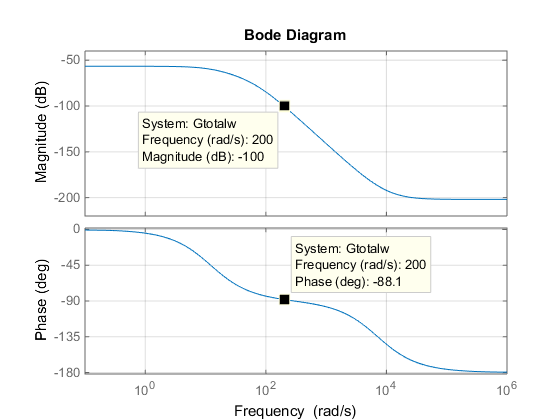
\includegraphics[scale=0.75]{diag_bode_planta_en_w.png}
	\caption{Diagrama de Bode de lazo abierto $GH_{T}(w)$ con $M=30\:kg$.}
	\label{fig:lugar-de-raices}
\end{figure}

\begin{figure}[H]
	\centering
	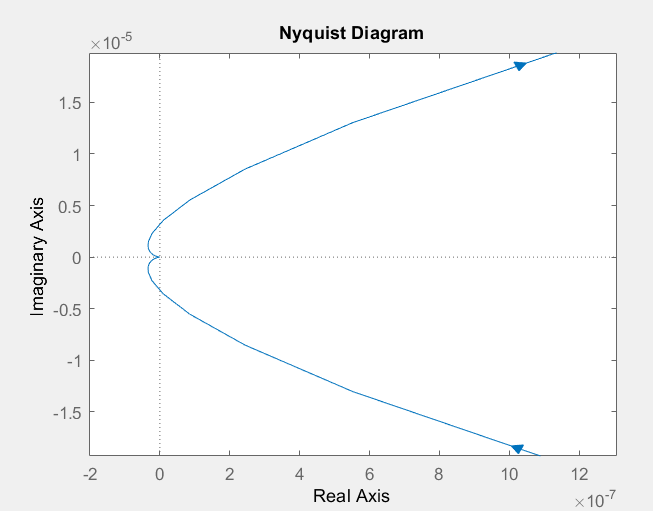
\includegraphics[scale=0.75]{Nyquist-lazo-abierto-digital.png}
	\caption{Diagrama de Nyquist de $GH_{T}(w)$ con $M=30\:kg$.}
	\label{fig:nyquist-lazo-abierto-digital}
\end{figure}

\noindent Dado que ${GH}_{T}(w)$ tiene un polo en el semiplano derecho, a partir del Nyquist se puede determinar:

\noindent Zona 1: $Z=N+P=0+1=1$ $\mathrm{\to}$ Inestable 

\noindent Zona 2: $Z=N+P=1+1=2$ $\mathrm{\to}$ Inestable

\noindent Dada la similitud de la planta en [w] con la planta del compensador analógico, se decide utilizar la misma estrategia de compensación con la misma ubicación de polos y ceros del compensador.	

\noindent Finalmente se llega a la transferencia del controlador:


 \begin{equation}  
 	G_c(w)=K*{[20.346*\frac{(w+44.3)}{(w+902.1)}]}^2
 \end{equation} 
 


\noindent En la figura \ref{fig:bode-compensado-para-k-1} se muestra el diagrama de bode de ${GH}_T(w)*G_c(w)$ con $K=1$. Se puede observar que la ganancia $K$ puede adoptar valores desde $64\:dB$ hasta $88.6\:dB$. Al considerar que el sistema debe soportar una masa variable entre $1\:kg$ y $30\:kg$, y que la ganancia de la transferencia de la planta para $1\:kg$ es de $5.5$ veces ($14\:dB$) mayor que para $30\:kg$, se debe adoptar una ganancia del compensador que mantenga la estabilidad para estos dos casos. Es decir, la ganancia m\'{i}nima es de $64\:dB$ y la m\'{a}xima es de $88.6\:dB - 14\:dB = 74.6\:dB$. Por lo tanto, se elige que el cruce por cero de la ganancia se encuentre ahora en $88\:rad/s$, lo que significa que $K=68.4\:dB\ \equiv \ 2630\:veces$.


\begin{figure}[H]
	\centering
	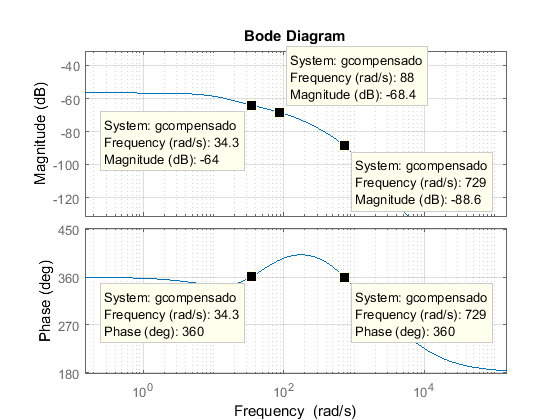
\includegraphics[scale=0.85]{Bode-compensado-para-k-1.png}
	\caption{Diagrama de Bode de $GH_T(w)*G_c(w)$ para $K=1$ y $M=30\:kg$.}
	\label{fig:bode-compensado-para-k-1}
\end{figure}


\noindent En la figura \ref{fig:bode-compensado-para-k-2630} se muestra el diagrama de Bode considerando la ganancia del compensador. En ella se puede observar que se  cumple con el criterio de estabilidad puesto que en el primer cruce por 0° la magnitud es mayor a $0\:dB$ y, en el segundo cruce, menor. Adem\'{a}s, en la figura \ref{fig:nyquist-para-k-2630} se puede ver que la forma del diagrama de Nyquist es como la deseada.

\begin{figure}[H]
	\centering
	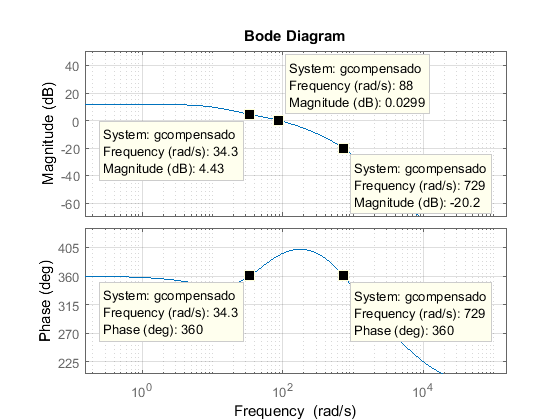
\includegraphics[scale=0.75]{Bode-compensado-para-k-2630.png}
	\caption{Diagrama de Bode de $GH_T(w)*G_c(w)$ para $K=2630$ y $M=30\:kg$.}
	\label{fig:bode-compensado-para-k-2630}
\end{figure}

\begin{figure}[H]
	\centering
	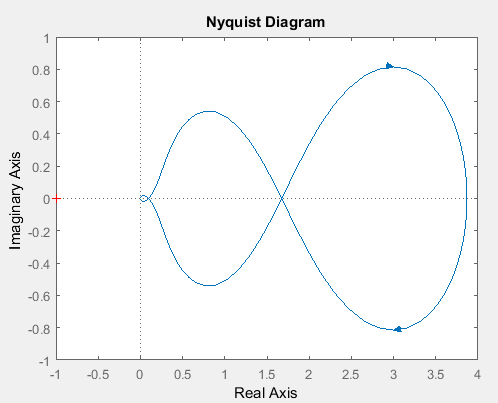
\includegraphics[scale=0.55]{Nyquist-para-k-2630.png}
	\caption{Diagrama de Nyquist de $GH_T(w)*G_c(w)$ para $K=2630$ y $M=30\:kg$.}
	\label{fig:nyquist-para-k-2630}
\end{figure}

\noindent En la figura \ref{fig:respuesta-al-escalon-para-M-30} se puede observar la respuesta al escal\'{o}n del sistema con masa de $30\:kg$.


\begin{figure}[H]
	\centering
	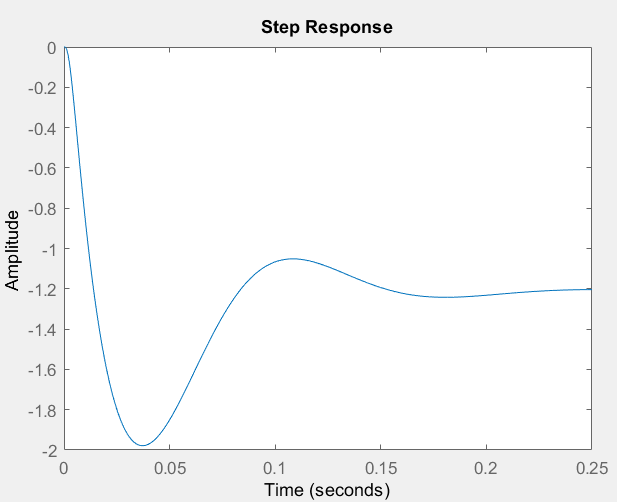
\includegraphics[scale=0.75]{Respuesta-al-escalon-para-M-30.png}
	\caption{Respuesta al escalón para $M=30\:Kg$.}
	\label{fig:respuesta-al-escalon-para-M-30}
\end{figure}

\subsection{Análisis de estabilidad con masa de 1 kg}

\noindent En esta secci\'{o}n se verifica la estabilidad del sistema  para el caso en que la masa sea de $1\:kg$, utilizando el compensador dise\~{n}ado para el caso de masa m\'{a}xima. Para ello, se analizan los diagramas de Bode y Nyquist mostrados en las figuras \ref{fig:bode-para-M-1Kg} y \ref{fig:nyquist-para-M-1Kg}. Adem\'{a}s, en la figura \ref{fig:respuesta-al-escalon-para-M-1Kg} puede observarse la respuesta al escal\'{o}n. A partir de ellos, es posible verificar que efectivamente el sistema resulta estable para todo el rango de masas en el que opera el sistema. 


\begin{figure}[H]
	\centering
	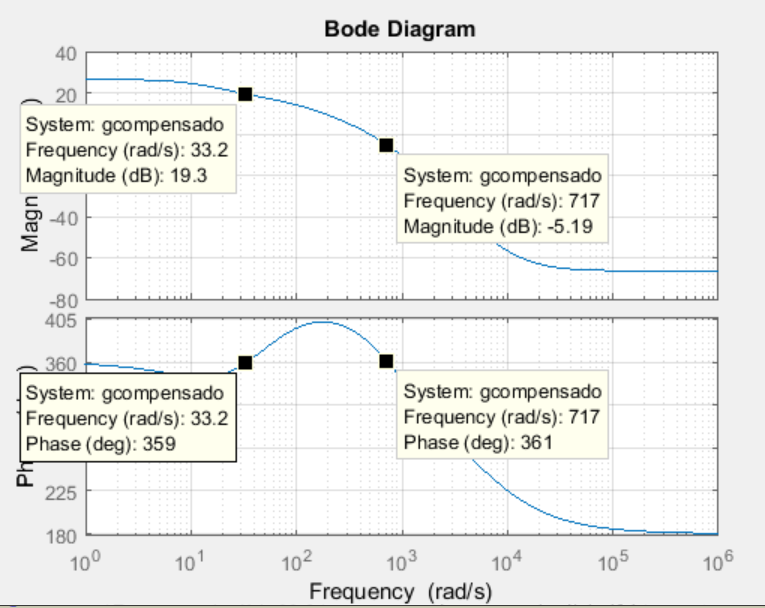
\includegraphics[scale=0.85]{Bode-para-M-1Kg.png}
	\caption{Diagrama de Bode de $GH_T(w)*G_c(w)$ para $M=1\:kg$.}
	\label{fig:bode-para-M-1Kg}
\end{figure}

\begin{figure}[H]
	\centering
	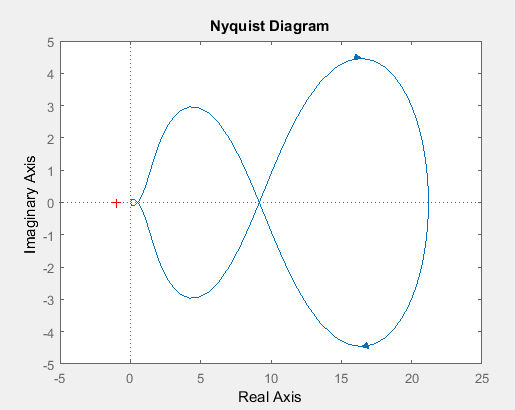
\includegraphics[scale=0.6]{Nyquist-para-M-1Kg.png}
	\caption{Diagrama de Nyquist de $GH_T(w)*G_c(w)$ para $M=1\:kg$.}
	\label{fig:nyquist-para-M-1Kg}
\end{figure}

\begin{figure}[H]
	\centering
	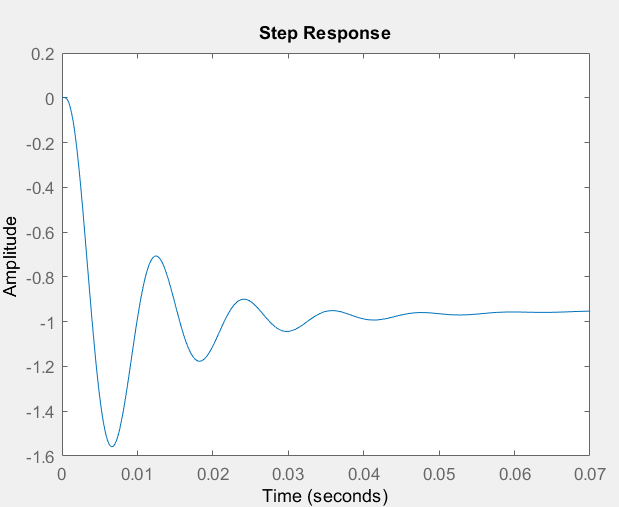
\includegraphics[scale=0.8]{Respuesta-al-escalon-para-M-1Kg.png}
	\caption{Respuesta al escalón para $M=1\:kg$.}
	\label{fig:respuesta-al-escalon-para-M-1Kg}
\end{figure}

\section{Diseño de lazo de realimentación externo}

\noindent Se plantea un lazo de realimentaci\'{o}n externo como se muestra en la  figura \ref{fig:diagrama-del-sistema-completo}.

\begin{figure}[H]
	\centering
	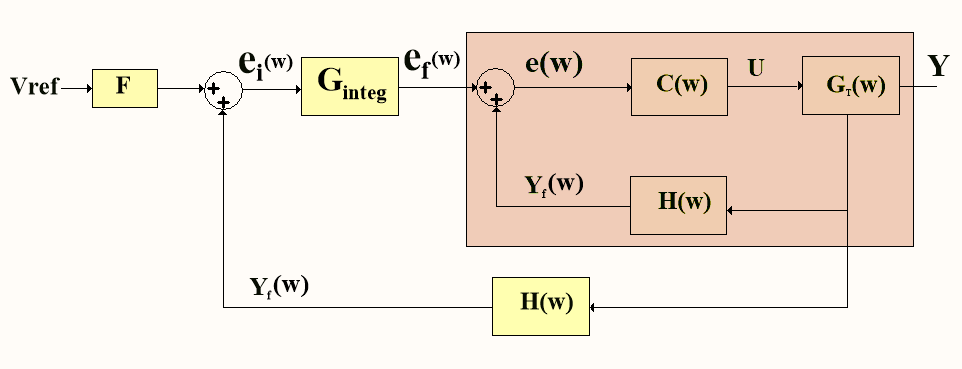
\includegraphics[scale=0.4]{Diagrama-del-sistema-completo.png}
	\caption{Diagrama del sistema completo.}
	\label{fig:diagrama-del-sistema-completo}
\end{figure}


\noindent En el lazo de realimentaci\'{o}n interno act\'{u}a el compensador por adelanto de fase dise\~{n}ado previamente y, en el externo, un controlador del tipo integral. De esta forma, se logra suavizar la respuesta al escal\'{o}n del sistema y eliminar el error en r\'{e}gimen permanente.


\noindent Para el an\'{a}lisis se considera $H(w)=1$ como realimentaci\'{o}n. La cadena de avance con masa de $30\:kg$ es:

\[G(W)[M=30]=Tlc(W)[M=30]*G_{integ}\] 

\noindent Se  plantea un compensador del tipo :

\[G_{integ}\ =\ k_{int}\ *\ \frac{1}{w}\] 

\noindent La ganancia del bloque de entrada (F) se establece igual a la ganancia del estimador (H) pero cambiada de signo, debido a que la transferencia de lazo cerrado tiene una inversi\'{o}n de fase. Por lo tanto, se toma $F=-H=-1$.

\noindent Inicialmente se adopta $k_{int} = 1$ para poder evaluar, por medio de lugar de ra\'{i}ces mostrado en la figura \ref{fig:lugar-de-raices-con-integrador}, la estabilidad del sistema. Para este lazo de realimentaci\'{o}n externo tambi\'{e}n debe utilizarse realimentaci\'{o}n positiva puesto que los polos de la TLC interna est\'{a}n en el semiplano izquierdo pero presenta una inversi\'{o}n de signo.


\begin{figure}[H]
	\centering
	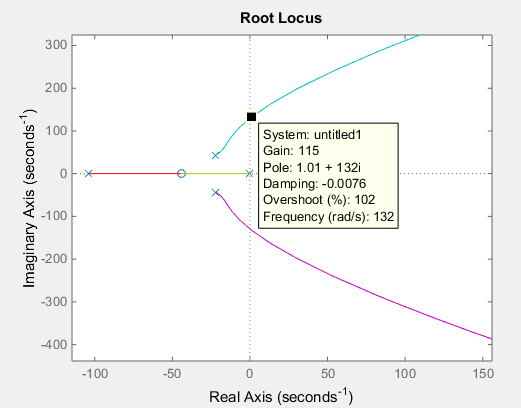
\includegraphics[scale=0.6]{Lugar-de-raices-con-integrador.png}
	\caption{Lugar de raíces con el integrador.}
	\label{fig:lugar-de-raices-con-integrador}
\end{figure}


\noindent En la figura \ref{fig:lugar-de-raices-con-integrador} se puede observar que, para que se mantenga la estabilidad del sistema, la ganancia del integrador ($K_{int}$) debe ser menor a 115. Por lo tanto, en la figura \ref{fig:respuesta-al-escalon-con-k-1-M-30} se muestra la respuesta al escal\'{o}n del sistema compensado con el integrador para una ganancia de $K_{int}=1$.  Es posible observar que, si bien no presenta oscilaciones, el tiempo de establecimiento es de aproximadamente $3\:s$. Por lo tanto, se decide aumentar el valor de ganancia hasta obtener una relaci\'{o}n aceptable entre el tiempo de respuesta y el sobrepico.


\begin{figure}[H]
	\centering
	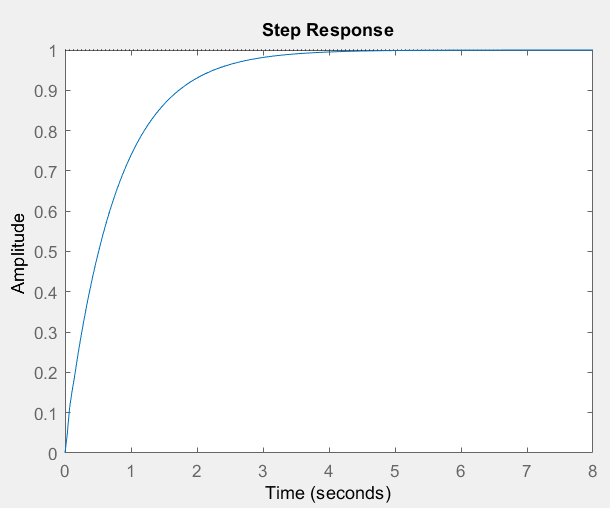
\includegraphics[scale=0.85]{Respuesta-al-escalon-con-k-1-M-30.png}
	\caption{Respuesta al escalón con integrador con $K_{int} =1$ y $M=30\:kg$.}
	\label{fig:respuesta-al-escalon-con-k-1-M-30}
\end{figure}


\noindent En la figura \ref{fig:respuesta-al-escalon-con-k-20-M-30}, se observa la respuesta al escal\'{o}n para una ganancia del integrador de $K_{int}=20$ que resulta en un tiempo de establecimiento de $0.22\:s$ y un \textsl{overshoot} de 4.41\%. Por lo tanto, se adopta este valor de ganancia para el dise\~{n}o del integrador.

\begin{figure}[H]
	\centering
	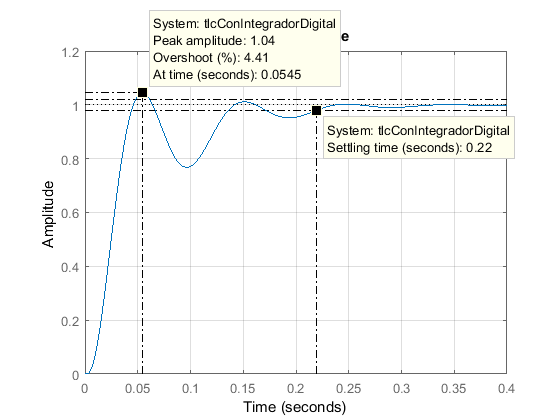
\includegraphics[scale=0.85]{Respuesta-al-escalon-con-k-20-M-30.png}
	\caption{Respuesta al escalón con integrador para $K_{int} =20$ y $M = 30\:kg$.}
	\label{fig:respuesta-al-escalon-con-k-20-M-30}
\end{figure}


\noindent La respuesta al escal\'{o}n cuando la masa es de $1\:kg$ se muestra en la figura \ref{fig:respuesta-al-escalon-con-k-20-M-1}. All\'{i} se puede observar que el tiempo de crecimiento es de $0.104\:s$ y el de establecimiento de $0.196\:s$. Adem\'{a}s, es posible notar que no presenta sobrepicos.



\begin{figure}[H]
	\centering
	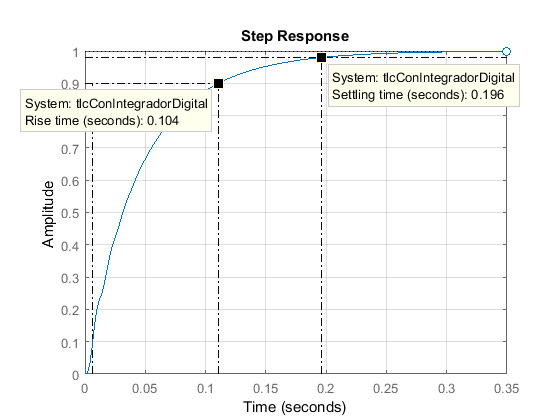
\includegraphics[scale=0.85]{Respuesta-al-escalon-con-k-20-M-1.png}
	\caption{Respuesta al escalón con integrador para $K_{int} =20$ y $M=1\:kg$.}
	\label{fig:respuesta-al-escalon-con-k-20-M-1}
\end{figure}


\section{Cálculo de los coeficientes del controlador}

\noindent Para implementar el algoritmo de control en el microcontrolador se aplica la transformada bilineal inversa a las transferencias del compensador por adelanto de fase $C(w)$ y al integrador $G_{integ}(w)$.

\noindent Por lo tanto, se obtiene:

\begin{equation} \label{GrindEQ__5_6_} 
	C(z)=\ \ \frac{U(z)}{e(z)}=\frac{8.6896*10^5(z-0.9877)^2}{\ (z-0.7757)^2}\  
\end{equation} 

\begin{equation} \label{GrindEQ__5_7_} 
	G_{integ}(z)=\frac{e_f(z)}{e_i(z)}\ =\frac{0.0028(\ z\ +\ 1)}{\ (z\ -\ 1)} 
\end{equation} 

\noindent Si se considera $H(z)=1$ se obtiene que:

\begin{equation} \label{GrindEQ__5_39_} 
	e(z)=e_f(Z)+Y_f(z) 
\end{equation} 

\begin{equation} \label{GrindEQ__5_40_} 
	e_i(z)=F*Vref+Y_f(z) 
\end{equation} 


\noindent Al aplicar la partir de las ecuaciones \ref{GrindEQ__5_6_} y \ref{GrindEQ__5_7_} se obtiene las expresiones a implementar en el microcontrolador:

\begin{equation} 
	\begin{aligned}\label{eq_U-coef}
	U[n]=&8.651*10^5e[n]-\ 1.709*10^6e[n-1]+\ 0.843*10^6e[n-2]+\\
		 &+1.5514\ U[n-1]-\ 0.60171U[n-2]\\ 
	\end{aligned}
\end{equation}

\begin{equation} \label{eq_e-coef} 
	e_f[n]=0.0028*e_i[n]\ +\ {0.0028*e}_i[n-1]+e_f[n-1] 
\end{equation} 


\noindent Luego, para dejar el algoritmo de control en funci\'{o}n de las entradas del sistema, se debe reemplazar en las ecuaciones \ref{eq_U-coef} y \ref{eq_e-coef} las expresiones mencionadas en las ecuaciones \ref{GrindEQ__5_10_} y \ref{GrindEQ__5_11_}

\begin{equation} \label{GrindEQ__5_10_} 
	e[n]=e_f[n]+Y_f[n] 
\end{equation} 

\begin{equation} \label{GrindEQ__5_11_} 
	e_i[n]=F*Vref+Y_f[n] 
\end{equation} 

\section{Conexi\'{o}n entre el PCB y el microcontrolador}

\noindent Se utiliza un conector tipo DB9 hembra como v\'{i}a de conexi\'{o}n para las distintas salidas y entradas digitales. Adem\'{a}s, en la placa se dispone de un led que se enciende cuando  se detecta una correcta conexi\'{o}n con el microcontrolador.







